%----------------------------------------------------------------------------------------
%	THE PULSE GENERATOR.
%----------------------------------------------------------------------------------------
\subsection{The pulse generator}


\begin{figure}[H]
\centering
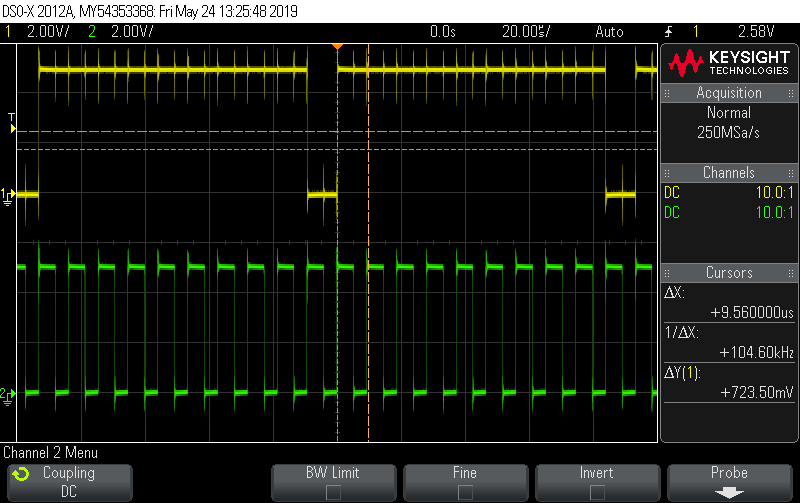
\includegraphics[width=.9\textwidth]{figures/scope_4.png}
\caption{Pulse generator circuit with yellow on 'PULSE 0' and green on 'OSC-OP', the interface between the oscillator and pulse generator.}
\label{fig:scope_4}
\end{figure}


\begin{figure}[H]
\centering
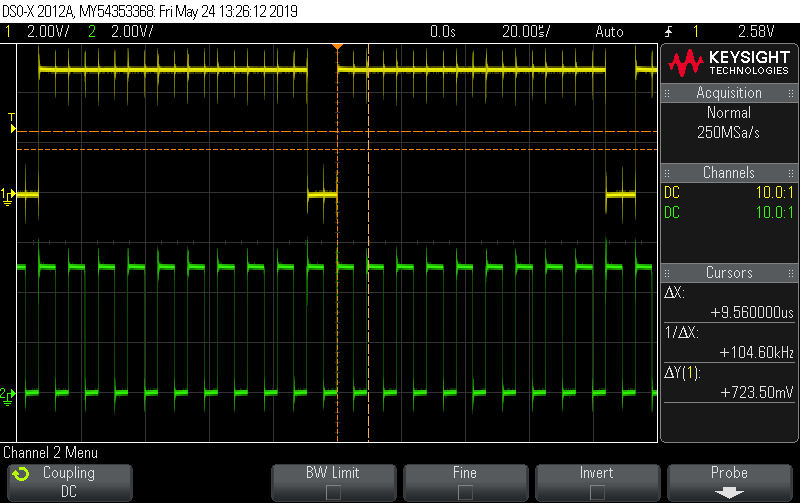
\includegraphics[width=.9\textwidth]{figures/scope_5.png}
\caption{Pulse generator circuit with yellow on 'PULSE 1' and green on 'OSC-OP', the interface between the oscillator and pulse generator.}
\label{fig:scope_5}
\end{figure}


\begin{figure}[H]
\centering
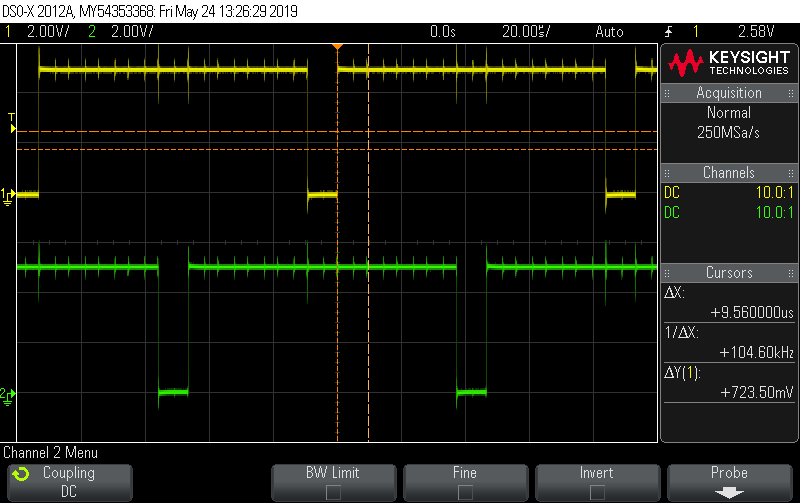
\includegraphics[width=.9\textwidth]{figures/scope_6.png}
\caption{Pulse generator circuit with yellow on 'PULSE 1' and green on 'PULSE 0'. It can be seen that the timing between these pulses is equal.}
\label{fig:scope_6}
\end{figure}

